\documentclass[noauthor]{ximera}
%handout:  for handout version with no solutions or instructor notes
%handout,instructornotes:  for instructor version with just problems and notes, no solutions
%noinstructornotes:  shows only problem and solutions

%% handout
%% space
%% newpage
%% numbers
%% nooutcomes

%I added the commands here so that I would't have to keep looking them up
%\newcommand{\RR}{\mathbb R}
%\renewcommand{\d}{\,d}
%\newcommand{\dd}[2][]{\frac{d #1}{d #2}}
%\renewcommand{\l}{\ell}
%\newcommand{\ddx}{\frac{d}{dx}}
%\everymath{\displaystyle}
%\newcommand{\dfn}{\textbf}
%\newcommand{\eval}[1]{\bigg[ #1 \bigg]}

%\begin{image}
%\includegraphics[trim= 170 420 250 180]{Figure1.pdf}
%\end{image}

%add a ``.'' below when used in a specific directory.

\newcommand{\RR}{\mathbb R}
\renewcommand{\d}{\,d}
\newcommand{\dd}[2][]{\frac{d #1}{d #2}}
\renewcommand{\l}{\ell}
\newcommand{\ddx}{\frac{d}{dx}}
\newcommand{\dfn}{\textbf}
\newcommand{\eval}[1]{\bigg[ #1 \bigg]}




\author{Jim Talamo}

\outcome{Find parameterizations of lines.}
\outcome{Determine the domain of a vector-valued function.}
\outcome{Determine if a curve intersects a surface nowhere, at finitely many points, or lies on the surface.}

\title[]{Calculus and Vector-Valued Functions}

\begin{document}
\begin{abstract}
\end{abstract}
\maketitle

\vspace{-0.5in}

\section{Discussion Questions}

\begin{problem} %Thanks to bart Snapp for this
The curve $\mathcal{C}$ traced out by  $\vec{p}(t)$ is shown below.

\begin{center}
\resizebox {5cm} {!} { 
    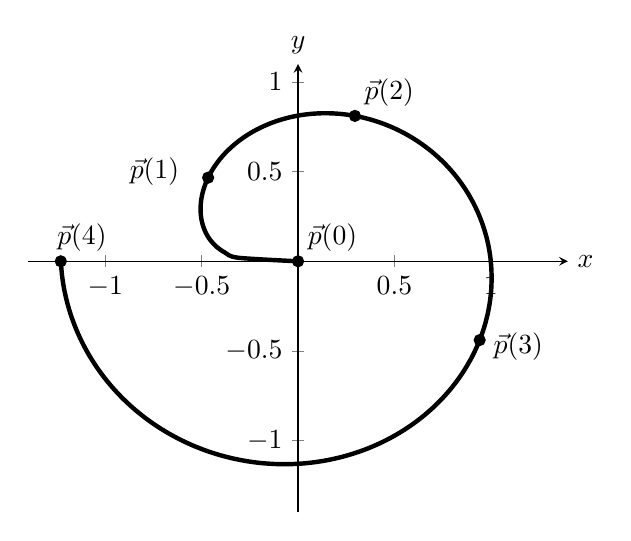
\begin{tikzpicture}
      \begin{axis}[
          xmin=-1.4, xmax=1.4, ymin =-1.4, ymax = 1.1,
          axis lines=center,  
          xlabel=$x$,  
          ylabel=$y$,  
          every axis y label/.style={at=(current axis.above origin),anchor=south},  
          every axis x label/.style={at=(current axis.right of origin),anchor=west}
        ]
        \addplot [black,ultra thick,domain=0:360,smooth,samples=100] ({-((x/180)^(.3))*cos(x)},{((x/180)^.3)*sin(x)});
        \node[above right,black] at (axis cs: 0,0) {$\vec{p}(0)$};
        \node[above right,black] at (axis cs: -1.3,0) {$\vec{p}(4)$};
        \node[above right,black] at (axis cs: {-((110/180)^(.3))*cos(110)},{((110/180)^.3)*sin(110)}) {$\vec{p}(2)$};
        \node[above left,black] at (axis cs: {-((45/180)^(.3))*cos(45)-.1},{((45/180)^.3)*sin(45)-.1}) {$\vec{p}(1)$};
        \node[above right,black] at (axis cs: {-((215/180)^(.3))*cos(215)+.1},{((215/180)^.3)*sin(215)}) {$\vec{p}(3)$};
        
        \addplot[color=black,fill=black,only marks,mark=*] coordinates{(-{((45/180)^(.3))*cos(45)},{((45/180)^.3)*sin(45)})};
        \addplot[color=black,fill=black,only marks,mark=*] coordinates{(-{((110/180)^(.3))*cos(110)},{((110/180)^.3)*sin(110)})};
        \addplot[color=black,fill=black,only marks,mark=*] coordinates{(-{((205/180)^(.3))*cos(205)},{((205/180)^.3)*sin(205)})};
        \addplot[color=black,fill=black,only marks,mark=*] coordinates{(-{((360/180)^(.3))*cos(360)},{((360/180)^.3)*sin(360)})};
        \addplot[color=black,fill=black,only marks,mark=*] coordinates{(0,0)};
        
      \end{axis}
    \end{tikzpicture}}
\end{center}

On the graph above, sketch the following.

I. The vector $\vec{p}(t)$ at $t=1$.  Make sure the tail of your vector is at the point associated to $\vec{p}(1)$.

II. A tangent vector for $\vec{p}(t)$ at $t=2$. Make sure the tail of your vector is at the point associated to $\vec{p}(2)$.

III. A vector in the same direction as $\vector{y(3),-x(3)}$ at $\vec{p}(3)$. Make sure the tail of your vector is at the point associated to $\vec{p}(3)$.



\begin{freeResponse}

I. From the picture, we see that $\vec{p}(1) \approx \vector{-.5,.5}$, so we draw the vector $\vector{-.5,.5}$ starting at the point associated to $\vec{p}(1)$.

II. To draw a tangent vector for $\vec{p}(t)$ at $t=2$, we draw a vector in the same direction as the curve.

III. From the picture, we note that $x(3) \approx -2 y(3)$ and $x(3)$ is positive, so a vector in the same direction as $\vector{-y(3),x(3)}$ will be parallel to $\vector{.5,1}$.


\begin{center}
\resizebox {6cm} {!} { 
    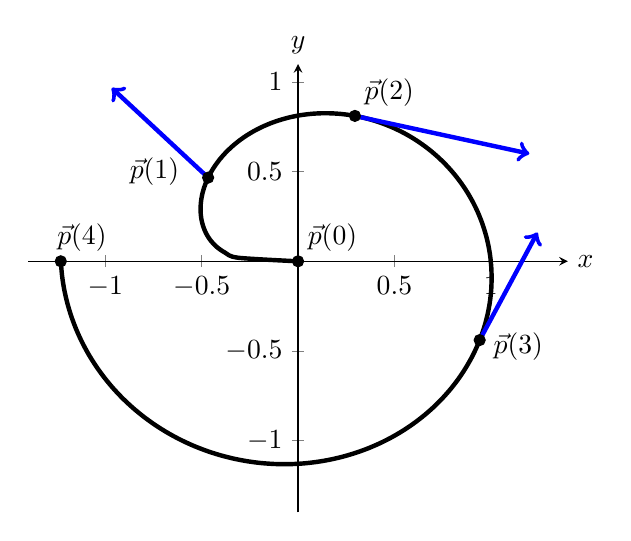
\begin{tikzpicture}
      \begin{axis}[
          xmin=-1.4, xmax=1.4, ymin =-1.4, ymax = 1.1,
          axis lines=center,  
          xlabel=$x$,  
          ylabel=$y$,  
          every axis y label/.style={at=(current axis.above origin),anchor=south},  
          every axis x label/.style={at=(current axis.right of origin),anchor=west},
          clip=false
        ]
        \addplot [black,ultra thick,domain=0:360,smooth,samples=100] ({-((x/180)^(.3))*cos(x)},{((x/180)^.3)*sin(x)});
        \node[above right,black] at (axis cs: 0,0) {$\vec{p}(0)$};
        \node[above right,black] at (axis cs: -1.3,0) {$\vec{p}(4)$};
        \node[above right,black] at (axis cs: {-((110/180)^(.3))*cos(110)},{((110/180)^.3)*sin(110)}) {$\vec{p}(2)$};
        \node[above left,black] at (axis cs: {-((45/180)^(.3))*cos(45)-.1},{((45/180)^.3)*sin(45)-.1}) {$\vec{p}(1)$};
        \node[above right,black] at (axis cs: {-((215/180)^(.3))*cos(215)+.1},{((215/180)^.3)*sin(215)}) {$\vec{p}(3)$};
        
        \addplot[color=black,fill=black,only marks,mark=*] coordinates{(-{((45/180)^(.3))*cos(45)},{((45/180)^.3)*sin(45)})};
        \addplot[color=black,fill=black,only marks,mark=*] coordinates{(-{((110/180)^(.3))*cos(110)},{((110/180)^.3)*sin(110)})};
        \addplot[color=black,fill=black,only marks,mark=*] coordinates{(-{((205/180)^(.3))*cos(205)},{((205/180)^.3)*sin(205)})};
        \addplot[color=black,fill=black,only marks,mark=*] coordinates{(-{((360/180)^(.3))*cos(360)},{((360/180)^.3)*sin(360)})};
        \addplot[color=black,fill=black,only marks,mark=*] coordinates{(0,0)};

        \addplot[blue,->,ultra thick] coordinates{(-{((45/180)^(.3))*cos(45)},{((45/180)^.3)*sin(45)}) (-{((45/180)^(.3))*cos(45)}-.5,{((45/180)^.3)*sin(45)+.5})};
        \addplot[blue,->,ultra thick] coordinates{(-{((110/180)^(.3))*cos(110)},{((110/180)^.3)*sin(110)})
          (1.2,.6)};
        \addplot[blue,->,ultra thick] coordinates{(-{((205/180)^(.3))*cos(205)},{((205/180)^.3)*sin(205)}) (-{((205/180)^(.3))*cos(205)+.3},{((205/180)^.3)*sin(205)+.6})};
      \end{axis}
    \end{tikzpicture}}

\end{center}

\end{freeResponse}


\end{problem}


%%%%%%%%%%%%%%%%%%%%%%%%%%%%%%%%%%%%%%%%%%%%%%%%%%%

\begin{problem}
Find a vector $\vec{v}$ parallel to the tangent line to $\vec{r}(t) = \vector{e^{2t},t^2-3t+1,\ln(1+2t^2)}$ at $t=0$.

\begin{freeResponse}
A vector $\vec{v}$ parallel to the tangent line will be $\vec{r}'(0)$.  We find $\vec{r}'(t) = \vector{2e^{2t},2t-3,\frac{4t}{1+2t^2}}$, so $\vec{v}=\vec{r}'(0) = \vector{2,-3,0}$.
\end{freeResponse}
\end{problem}
%%%%%%%%%%%%%%%%%%%%%%%%%%%%%%%%%%%%%%%%%%%%%%%%%%%


\begin{problem}
In the following statements, properties of a differentiable vector-valued function $\vec{r}(t)$ are given.  Determine if the following statements are true or false and explain your reasoning.

I.  If it is known that $| \vec{r}(t) | = t^2$.  Then,  $| \vec{r}  ' (t) | = 2t$.

II. If $\vec{r}(t)$ is a unit vector for all $t$.  Then $\vec{r}  ' (t)$  is a unit vector for all $t$. 

III. If $\vec{r}(t)$ is a unit vector for all $t$, then $\dfrac{d}{dt} |\vec{r}(t) | =0$.

IV. If $\vec{r}(0)=\vector{1,2,0}$, and $\vec{r}'(t)=\vec{0}$, then $\vec{r}(t) = \vector{1,2,0}$ for all $t$.

 \begin{freeResponse}
By introducing a parameter to describe a curve, we introduce a notion of how to trace out the curve.  We thus have reason to think of the quantities of speed and acceleration.

\begin{itemize}
\item $\vec{r}(t)$ gives the position $(x,y,z)$ at a particular time $t$.
\item $|\vec{r}(t)|$ gives the distance the corresponding point $(x,y,z)$ is from the origin.
\item $\vec{r}'(t) = \frac{\d}{\d t} \left[\vphantom{\bigg|} \vec{r}(t) \right]$ is the velocity.
\item  $\left|\vec{r}'(t)\right| = \left|\vphantom{\bigg|}  \frac{\d}{\d t}\left[\vec{r}(t) \right]\right|$ is the speed.
\end{itemize}
Pay close attention to the difference between the last two expressions.  Before tackling the true and false questions below, recall that the same curve can be traced out in many ways.  

 \textbf{I. False}
 
\begin{explanation}
Intuitively, $| \vec{r}(t) | = t^2$ tells us that the distance from the origin a point $(x(t),y(t),z(t))$ is at time $t$.  Knowing this distance should have no relationship with exactly how fast the point on the curve is moving.
 
 For a specific counterexample, take $\vec{r}(t)=\vector{t^2\cos(t),t^2\sin(t)}$.  Then, $|\vec{r}(t)| = t^2$, but $\vec{r}'(t) = \vector{2t\cos(t)-t^2\sin(t), 2t\sin(t)+t^2\cos(t)}$.  Now, if $|\vec{r}'(t)|=2t$ for all $t$, it certainly should be true that $|\vec{r}'(\pi)|=2\pi$ (where the choice $t=\pi$ was made since we can check whether $|\vec{r}'(t)| = 2t$ easily there).  However, $\vec{r}(\pi) = \vector{-2\pi,-\pi^2}$, so  $|\vec{r}'(\pi)| = \sqrt{4\pi^2+\pi^4} \neq 2 \pi$.
\end{explanation}
 
 \textbf{II. False} 
 
 \begin{explanation}
 Intuitively, if $\vec{r}(t)$ is a unit vector for all time $t$, this means that the point on the curve at any time $t$ is $1$ unit away from the origin.  In three dimensions, this means that the point could be moving along a sphere of radius $1$.  No matter how quickly it is moving, as long as it stays on the sphere, it will be $1$ unit away from the origin.  Thus, knowing the magnitude of $\vec{r}(t)$ should not give an information about the magnitude of $\vec{r}'(t)$ (i.e. the speed).
 
 For a specific counterexample, take $\vec{r}(t) = \vector{\cos(\omega t),\sin(\omega t)}$ (this describes a particle moving counterclockwise in a circle with angular speed $\omega$).  You can check the following.
 
 \begin{itemize}
 \item $|\vec{r}(t)| = 1$.
 \item $\vec{r}'(t) = \vector{-\omega \sin(\omega t), \omega \cos(\omega t)}$, so $|\vec{r}'(t)| = \omega$.
 \end{itemize}
 \end{explanation}

 
 \textbf{III. True}

\begin{explanation}
Make sure to pay attention to what we are given and being asked to find.  We are given that the distance the point on the curve is from the origin is always $1$.  The derivative $\dfrac{\d}{\d t} |\vec{r}(t) |$ will give us how this magnitude changes in time, so it must be $0$.  Note in particular that $\dfrac{\d}{\d t} |\vec{r}(t) |$ is \emph{not} the speed.  Said more explicitly,

\[
\frac{\d}{\d t} \left[\vphantom{\bigg|} |\vec{r}(t)| \right] \neq |\vec{r}'(t)|.
\]
\end{explanation}

\textbf{IV. True}

\begin{explanation}
Intuitively, the derivative $\vec{r}'(t)$ will provide information about how the vector $\vec{r}(t)$ changes in time.  Vectors have both magnitudes and directions, and we know that $\vec{r}'(t)=\vec{0}$ tells us that nothing about either of these quantities will change.

Computationally, note that $\int \vec{r}'(t) \d t = \int \vector{0,0,0} \d t$, so

\[
\vec{r}(t) = \vector{C_1,C_2,C_3}.
\]

From the above, $\vec{r}(0) = \vector{C_1,C_2,C_3}$. Since we also have$\vec{r}(0) = \vector{1,2,0}$, we must have $C_1=1$, $C_2=2$, $C_3=0$, so $\vec{r}(t) = \vector{1,2,0}$ for all $t$.
\end{explanation}

\end{freeResponse}
 
\end{problem}



%%%%%%%%%%%%%%%%%%%%%%%%%%%%%%%%%%%%%%%%%%%%%%%%%%%

\section{Group Work}

\begin{problem}
Consider the curve $\mathcal{C} = \left\{(x,y) \in \R^2 ~ \bigg| ~ x=4-y^2\right\}$ .

I. Find a Cartesian representation of the tangent line at $y=1$.

II. Require that $y(t) =2t$.  Give a parametric description of $\mathcal{C}$ with this choice of $y(t)$ and find a parametric description of the tangent line at  $y=1$. 

III. Do the answers to Part I and Part II describe the same line?


 \begin{freeResponse}
 \textbf{I.} Differentiating gives $\frac{\d x}{\d y} = -2y$, so $\frac{\d x}{\d y} = -2$, and thus, $\frac{\d y}{\d x} = -\frac{1}{2}$.  Note also that when $y=1$, $x=3$.  The equation of the tangent line is thus found from point-slope form.
 
 \begin{align*}
 y-y_0 &= m_{\tan}(x-x_0) \\
 y-1 &= -\frac{1}{2} (x-3) \\
 y &= -\frac{1}{2}x+\frac{5}{2}.
 \end{align*}
 
 \textbf{II.}  If $y(t)=2t$, note that $x(t) =4-(2t)^2 = 4-4t^2$.  Hence, the position vector $\vec{r}(t) = \vector{4-4t^2,2t}$, and we have that $y=1$ when $t=\frac{1}{2}$.  To give a parameterization of the tangent line at $t=\frac{1}{2}$, we need a vector parallel to the line and a point $P_0$ on the line.
 
 \begin{itemize}
 \item A vector $\vec{v}$ parallel to the tangent line is $\vec{r}'\left(\frac{1}{2}\right)$. We find $\vec{r}'(t) = \vector{-8t,2}$, so $\vec{v} =\vec{r}'\left(\frac{1}{2}\right) =\vector{-4,2}$.
 \item A point on the line can be found from $\vec{r}\left(\frac{1}{2}\right) = \vector{3,1}$.
 \end{itemize}
 
 Thus a parametric description for the tangent line is
 
 \[
 \vec{l}(t) = \vec{v}t+\vec{P}_0 = \vector{-4,2}t+ \vector{3,1} = \vector{-4t+3,2t+1}.
 \]
 
 \textbf{III.} To check to see if the representations describe the same tangent line, we note from the answer to Part II that $x(t) = -8t+3$ and $y(t) = 2t+1$.  We thus need to substitute these into the description of the line  $y = -\frac{1}{2}x+\frac{5}{2}$ found in Part I and check if they agree.  Note that
 
 \[
 -\frac{1}{2}[x(t)]+\frac{5}{2} =  -\frac{1}{2}[-4t+3]+\frac{5}{2} = 2t -\frac{3}{2}+\frac{5}{2} = 2t+1.
 \]
 Thus, the answers to each part describe the same line.
 
 \begin{remark}
 This problem emphasizes an important point.  The tangent line to a curve at a specific point is a property of the curve itself.  It should \emph{not} depend on the way we choose to represent the curve.
 \end{remark}
 
 \end{freeResponse}
\end{problem}

%%%%%%%%%%%%%%%%%%%%%%%%%%%%%%%%%%%%%%%%%%%%%%%%%%%


\begin{problem}
The curve $\mathcal{C}$ is traced out by the vector-valued function \[ \vec{r}(t) = \vector{4+3t, t^2+3,4t-3}, -\infty < t <\infty.\]   


I. Find all $t$-values for which $\vec{r}(t)$ and $\vec{r}'(t)$ are orthogonal.

II. Find all $t$-values for which $|\vec{r}'(t)| = 4$ or explain why there are none. 

III. Find the unit tangent vector $\uvec{T}(t)$.  

IV.  Without calculating them, do you expect $\frac{\d}{\d t} |\uvec{T}(t)|$ or $|\uvec{T}'(t)|$ to be $0$?  Check your intuition by calculating them.
 
 \begin{freeResponse}  We note that $\vec{r}'(t) = \vector{3,2t,4}$.
 
 \textbf{I.} We must find all $t$-values for which $\vec{r}(t) \dotp \vec{r}'(t) = 0$.
 
 \begin{align*}
 \vec{r}(t) \dotp \vec{r}'(t) = \vector{4+3t, t^2+3,4t-3} \dotp  \vector{3,2t,4} &= 12+9t+2t^3+6t+16t-12 =2t^3+31t\\
 &= t(2t^2+31)
 \end{align*}
 
 This is only $0$ when $t=0$.
 
 \textbf{II.} Note that $|\vec{r}(t)| = \sqrt{(3)^2+(2t)^2+(4)^2} = \sqrt{25+4t^2} > 5$ for all $t$.  Thus, there are no $t$-values for which $|\vec{r}'(t)| = 4$.
 
 \textbf{III.} A vector parallel to the tangent line for a given $t$-value can be found by evaluating $\vec{r}'(t)$ at the same $t$-value.  However, $\vec{r}'(t)$ need not be a unit vector, but since $|\vec{r}'(t)| \neq 0$, we can always construct a unit vector the usual way.
 
 \[
 \uvec{T}(t) = \frac{\vec{r}'(t)}{|\vec{r}'(t)|} = \frac{\vector{3,2t,4}}{ \sqrt{25+4t^2}}.
 \]
 
 \textbf{IV.} The unit tangent vector has constant magnitude, so $\frac{\d}{\d t} |T(t)|$ must be $0$.  However, it appears that $\uvec{T}(t)$ is changing in time, so likely, $|\uvec{T}'(t)| \neq 0$.
 
 Note by definition, $\frac{\d}{\d t} |T(t)| = \frac{\d}{\d t} \left[ \vphantom{\bigg|}|T(t)|\right] = \frac{\d}{\d t}[1] =0$.  A routine application of the quotient rule and some tedious algebra gives that 
 
 \[
 \uvec{T}'(t) = \frac{1}{(25+4t^2)^{3/2}}\vector{-12t, 50 , -16t}. 
 \]
 After more algebra, 
 \[
 |\uvec{T}'(t)| = \frac{10}{4t^2+25}.
 \] 
 \end{freeResponse}
\end{problem}

%%%%%%%%%%%%%%%%%%%%%%%%%%%%%%%%%%%%%%%%%%%%%%%%%%%

%FINISH THIS LATER

%\begin{problem}
%Suppose that $\vec{r}(t)$ is a vector-valued function and $|\vec{r}(t)| = t^2+1$.  
%
%I. Determine all times $t$ for which $\vec{r}(t)$ and $\vec{r}'(t)$ are orthogonal or explain why they are never orthogonal.
%
%II. Construct a specific example of a function $\vec{r}(t)$ for which $|\vec{r}(t)| = t^2+1$.  Then, verify your answer to Part I for the function that you found.  
% 
% \begin{freeResponse}
% 
% \end{freeResponse}
%\end{problem}

%%%%%%%%%%%%%%%%%%%%%%%%%%%%%%%%%%%%%%%%%%%%%%%%%%%


\end{document}
